\documentclass[a4paper,12pt]{article}
\usepackage[margin=2cm]{geometry}
\usepackage{amsmath}
\usepackage[x11names]{xcolor}
\usepackage[colorlinks, citecolor=DodgerBlue2, linkcolor=Purple4, urlcolor=DeepPink2]{hyperref}
\usepackage[bitstream-charter]{mathdesign}
\usepackage{graphicx}
\usepackage[utf8]{inputenc}
\usepackage{nicefrac}
\usepackage[detect-all=true]{siunitx}
\usepackage{float}
\usepackage{enumitem}
\usepackage{physics}
\usepackage{wrapfig}
\setlength{\parindent}{0pt}
\sisetup{separate-uncertainty}

\setlist{nolistsep}
\setlist{noitemsep}
\usepackage{tikz}
\usepackage{tikz-3dplot}
\usetikzlibrary{positioning}
\usetikzlibrary{arrows.meta}
\usetikzlibrary{shapes.symbols}
\usetikzlibrary{shapes.geometric}
\usetikzlibrary{3d}
\tdplotsetmaincoords{65}{115}
\tikzset{math3d/.style=
  {x= {(-0.353cm, -0.353cm)}, z={(0cm, 1cm)},y={(1cm, 0cm)}}}

\newcommand{\BFO}{BiFeO\textsubscript{3}\ }

\title{BFO-ator Manual}
\author{Aurore Finco\\ \href{mailto:aurore.finco@umontpellier.fr}{aurore.finco@umontpellier.fr}\\ \textit{Laboratoire Charles Coulomb, CNRS and University of Montpellier, France}}
\date{\today}

\begin{document}

\maketitle

This program computes the stray field profile from the cycloid in \BFO, as it is measured with NV center magnetometry. Three cases are considered, and correspond to the three available tabs:
\begin{itemize}
  
\item The type 1 (bulk-like) cycloid in (001)-oriented \BFO
\item The type 2 (exotic) cycloid in (001)-oriented \BFO
\item The type 1 (bulk-like) cycloid in (111)-oriented \BFO
\end{itemize}
In each tab, you can enter the parameters in the left section on the window. These parameters are detailed in the following sections. In the right part of the window, the corresponding profiles are plotted. You can select which magnetic field components you would like to plot with the tick boxes. With the save button, you can export these profiles in .txt format. Above the plots, the amplitude and apparent period indicated correspond to the $B_\text{NV}$ component.
\begin{center}
  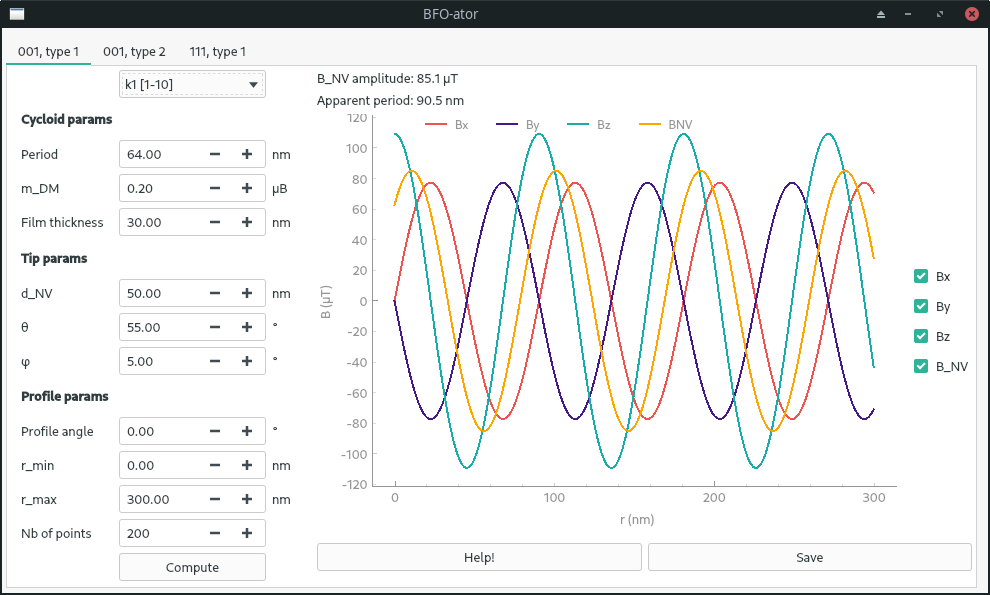
\includegraphics[width=15cm]{BFO-ator_window.png}
\end{center}

\clearpage
\section{Tab 001, type 1}
\subsection{Geometry and parameters}

\begin{wrapfigure}[22]{l}{8cm}
  \centering
  \begin{tikzpicture}[tdplot_main_coords]
    \def\c{2.7}
        \draw[thin, gray] (\c, 0, 0)--(\c, \c, 0)--(\c, \c, \c)--(\c, 0, \c)--cycle;
        \draw[thin, gray] (\c, \c, 0)--(0, \c, 0)--(0, \c, \c)--(\c, \c, \c);
        \draw[thin, gray] (\c, 0, \c)--(0, 0, \c)--(0,\c, \c);
        \draw[dashed, thin, gray] (\c, 0, 0)--(0, 0, 0)--(0,\c, 0);
        \draw[dashed, thin, gray] (0, 0, \c)--(0, 0, 0);
        \draw[orange, line width=2pt, stealth-stealth](0, 0, \c)--++(0, \c, -\c) node[node font=\large, above right]{$\vec{k}_3 [0\bar{1}1]$};
        \draw[gray!70, line width=3pt, -Triangle] (0, 0, 0)--(\c, \c, \c )node[gray, node font=\large, above=2mm, fill=white, fill opacity= 0.7,inner sep=0.5pt]{$\vec{P} [111]$};
        \draw[violet, line width=2pt, stealth-stealth](0, \c, 0)--++(\c, -\c, 0) node[node font=\large, below]{$\vec{k}_1 [1\bar{1}0]$};
        \draw[red, line width=2pt, stealth-stealth](\c, 0, 0)--++(-\c, 0, \c) node[node font=\large, below left=4mm, fill=white, fill opacity= 0.7,inner sep=0.5pt]{$\vec{k}_2 [\bar{1}01]$};

        \begin{scope}[xshift=3cm, yshift=-1.75cm]
          \draw[-stealth] (0, 0, 0)--(0, 0, 1)node[right]{$z$};
          \draw[-stealth] (0, 0, 0)--(1, 0, 0)node[below]{$x$};
          \draw[-stealth] (0, 0, 0)--(0, 1, 0)node[below]{$y$};
        \end{scope}


        \begin{scope}
          \def\z{7}
          \draw[thin, fill=cyan!10] (\c, 0, \z) --++ (2*\c, 0, 0) --++ (0, 2*\c, 0) --++ (-2*\c, 0, 0) -- cycle;
          \node[align=center] at (5, -0.5, 7.5){imaging\\ plane};
          \draw[-stealth] (1.5*\c, \c, \z)--++(\c, 0, 0)node[below left]{$x$};
          \draw[-stealth] (2*\c, 0.5*\c, \z)--++(0, \c, 0)node[right]{$y$};
          \draw[ultra thick, Blue4] (1.5*\c, 0.25*\c, \z)--++(\c, 1.5*\c, 0);
          \node[Blue4, node font=\footnotesize, rotate=-36] at (1.45*\c, 0.4*\c, \z){profile};
          \draw[Blue4] (2.3*\c, \c, \z) to [bend right] (2.15*\c, 1.25*\c, \z);
          \node[Blue4, align=center, node font=\footnotesize] at (2.6*\c, 1.3*\c, \z) {profile\\[-3pt] angle};
          
        \end{scope}

        \begin{scope}
          \def\d{8}

          \draw[-stealth] (1, 1, \d-1.25)--++(0,0,2.5);
          \draw[SpringGreen3] (1, 1, \d+0.75) to [bend left] (1, 1.5, \d+0.45);
          \node[SpringGreen3] at (1.2, 1.5, \d+1.2){$\theta$};
          \draw[-stealth] (-1.25, 1, \d)--++(2.5,0,0);
          \draw[-stealth] (1, -0.5, \d)--++(0,3,0);
          \draw[SpringGreen3, line width=4pt, -stealth] (-1, -1, \d-2)--++(4, 4, 4);
          \node[fill=SpringGreen3, circle] at (1, 1, \d){};
          \node[SpringGreen3, node font={\large,\bf}] at (1.5, 0.5, \d+0.5){NV};
          \draw[SpringGreen3, dashed] (3, 3, \d+2)--(3, 3, \d)--(1,1,\d);
          \draw[SpringGreen3] (2.5, 1, \d) to [bend right] (2, 2, \d);
          \node[SpringGreen3] at (2.5, 1.25, \d-0.5){$\varphi$};
          \draw[-stealth] (1, 1, \d)--++(2.5,0,0);
        \end{scope}

     \end{tikzpicture}
  \caption{Geometry of the considered type 1 cycloid in (001)-oriented \BFO}
\end{wrapfigure}


\textbf{Parameters:}

\begin{itemize}
\item Cycloid parameters
  \begin{itemize}
  \item Period: cycloid period in \si{\nano\meter}, \textbf{not}\\ projected onto the imaging plane,\\ usually around \SI{64}{\nano\meter}
  \item m\_DM: canted magnetic moment,\\ in $\mu_B$
  \item Film thickness: in \si{\nano\meter}
  \end{itemize}
  
\item Tip parameters
  \begin{itemize}
  \item d\_NV: distance between the NV center and the surface, in \si{\nano\meter}
  \item $\theta$: polar angle of the NV orientation, in~°
  \item $\varphi$: azimuthal angle of the NV\\ orientation, in~°
  \end{itemize}
 
\item Profile parameters
  \begin{itemize}
  \item Profile angle: direction of the\\ measured profile, in~°
  \item r\_min, r\_max: start and stop \\coordinates of the profile, in \si{\nano\meter}
  \item Nb of points: Number of data points along the profile
  \end{itemize}
\end{itemize}

\vspace*{3mm}

\subsection{Analytical expression}

\subsubsection{Cycloid propagating along $\vec{k}_1$}

 \begin{equation*}
    \left \lbrace
      \begin{aligned}
        B_{x} & = \frac{\mu_0 \ m_\text{DM}}{\sqrt{3} V}  e^{-k d_\text{NV}} \frac{1-e^{-kt}}{1-e^{-ka}} \sinh \left(\frac{ka}{2}\right) \sin\left( \frac{k}{\sqrt{2}} (x-y)\right) \\
        B_{y} & = -\frac{\mu_0 \ m_\text{DM}}{\sqrt{3} V}  e^{-k d_\text{NV}} \frac{1-e^{-kt}}{1-e^{-ka}} \sinh \left(\frac{ka}{2}\right) \sin\left( \frac{k}{\sqrt{2}} (x-y)\right) \\
        B_{z} & = \sqrt{\frac{2}{3}} \frac{\mu_0 \ m_\text{DM}}{V}  e^{-k d_\text{NV}} \frac{1-e^{-kt}}{1-e^{-ka}} \sinh \left(\frac{ka}{2}\right) \cos\left( \frac{k}{\sqrt{2}} (x-y)\right) \\
      \end{aligned}
    \right.
  \end{equation*}
  where $a$ is the \BFO lattice parameter and $t$ the film thickness.

  \clearpage
  \subsubsection{Cycloid propagating along $\vec{k}_2$}

\begin{equation*}
    \left \lbrace
      \begin{aligned}
        B_x & = - \frac{A}{\sqrt{2}} \left(  \Re{S}-
          \Im{S} \right)\\
        B_y &= 0\\
        B_z & =  \sqrt{2} \ A \Re{S}\\
      \end{aligned}
    \right.
  \end{equation*}

  \vspace*{10mm}

  with:
  \[A = \frac{\mu_0 m_\text{DM}}{\sqrt{3}V}\sinh(\frac{ka}{2\sqrt{2}})\] 
  \[S = e^{\nicefrac{-kd_\text{NV}}{\sqrt{2}}} e^{\nicefrac{ik(x-d_\text{NV})}{\sqrt{2}}}   \        \frac{1-e^{\nicefrac{-kt(1+i)}{\sqrt{2}}}}{1-e^{\nicefrac{-ka(1+i)}{\sqrt{2}}}} \]

   where $a$ is the \BFO lattice parameter and $t$ the film thickness.

   \subsubsection{Cycloid propagating along $\vec{k}_3$}

\begin{equation*}
    \left \lbrace
      \begin{aligned}
        B_x &= 0\\
        B_y & = - \frac{A}{\sqrt{2}} \left(  \Re{S}-
          \Im{S} \right)\\
        B_z & =  \sqrt{2} \ A \Re{S}\\
      \end{aligned}
    \right.
  \end{equation*}

  \vspace*{10mm}

  with 
  \[ A = \frac{\mu_0 m_\text{DM}}{\sqrt{3}V}\sinh(\frac{ka}{2\sqrt{2}})\]
  \[S = e^{\nicefrac{-kd_\text{NV}}{\sqrt{2}}} e^{\nicefrac{ik(y-d_\text{NV})}{\sqrt{2}}}   \        \frac{1-e^{\nicefrac{-kt(1+i)}{\sqrt{2}}}}{1-e^{\nicefrac{-ka(1+i)}{\sqrt{2}}}}\]

  where $a$ is the \BFO lattice parameter and $t$ the film thickness.
  
\clearpage
\section{Tab 001, type 2}
\subsection{Geometry and parameters}

If the cycloid propagates along $\vec{k'}_3 [11\bar{2}]$, the canted magnetic moments are in the surface plane and therefore the cycloid does not produce stray field. Hence the introduction of the deviation angle $\alpha$.

\begin{wrapfigure}[23]{l}{8cm}
  \centering
  \begin{tikzpicture}[tdplot_main_coords]
    \def\c{2.7}
        \draw[thin, gray] (\c, 0, 0)--(\c, \c, 0)--(\c, \c, \c)--(\c, 0, \c)--cycle;
        \draw[thin, gray] (\c, \c, 0)--(0, \c, 0)--(0, \c, \c)--(\c, \c, \c);
        \draw[thin, gray] (\c, 0, \c)--(0, 0, \c)--(0,\c, \c);
        \draw[dashed, thin, gray] (\c, 0, 0)--(0, 0, 0)--(0,\c, 0);
        \draw[dashed, thin, gray] (0, 0, \c)--(0, 0, 0);
         \draw[violet, line width=2pt, stealth-stealth](0, \c, 0.5*\c)--++(\c, -0.5*\c, -0.5*\c) node[node font=\large, below]{$\vec{k'}_1 [\bar{2}11]$};
         \draw[red, line width=2pt, stealth-stealth](0.5*\c, \c, 0)--++(0.5*\c, -\c, 0.5*\c) node[node font=\large, left, fill=white, fill opacity= 0.7,inner sep=0.5pt]{$\vec{k'}_2 [1\bar{2}1]$};
        \draw[orange, line width=2pt, stealth-stealth](0.5*\c, 0.5*\c, 0)--++(-0.5*\c, -0.5*\c, \c) node[fill=white, fill opacity= 0.7,inner sep=0.5pt, node font=\large, below left]{$\vec{k'}_3 [11\bar{2}]$};
        \draw[gray!70, line width=3pt, -Triangle] (0, 0, 0)--(\c, \c, \c )node[gray, node font=\large, above=2mm, fill=white, fill opacity= 0.7,inner sep=0.5pt]{$\vec{P} [111]$};
       
       

        \begin{scope}[xshift=3cm, yshift=-1.75cm]
          \draw[-stealth] (0, 0, 0)--(0, 0, 1)node[right]{$z$};
          \draw[-stealth] (0, 0, 0)--(1, 0, 0)node[below]{$x$};
          \draw[-stealth] (0, 0, 0)--(0, 1, 0)node[below]{$y$};
        \end{scope}


        \begin{scope}
          \def\z{7}
          \draw[thin, fill=cyan!10] (\c, 0, \z) --++ (2*\c, 0, 0) --++ (0, 2*\c, 0) --++ (-2*\c, 0, 0) -- cycle;
          \node[align=center] at (5, -0.5, 7.5){imaging\\ plane};
          \draw[-stealth] (1.5*\c, \c, \z)--++(\c, 0, 0)node[below left]{$x$};
          \draw[-stealth] (2*\c, 0.5*\c, \z)--++(0, \c, 0)node[right]{$y$};
          \draw[ultra thick, Blue4] (1.5*\c, 0.25*\c, \z)--++(\c, 1.5*\c, 0);
          \node[Blue4, node font=\footnotesize, rotate=-36] at (1.45*\c, 0.4*\c, \z){profile};
          \draw[Blue4] (2.3*\c, \c, \z) to [bend right] (2.15*\c, 1.25*\c, \z);
          \node[Blue4, align=center, node font=\footnotesize] at (2.6*\c, 1.3*\c, \z) {profile\\[-3pt] angle};
          
        \end{scope}

        \begin{scope}
          \def\d{8}

          \draw[-stealth] (1, 1, \d-1.25)--++(0,0,2.5);
          \draw[SpringGreen3] (1, 1, \d+0.75) to [bend left] (1, 1.5, \d+0.45);
          \node[SpringGreen3] at (1.2, 1.5, \d+1.2){$\theta$};
          \draw[-stealth] (-1.25, 1, \d)--++(2.5,0,0);
          \draw[-stealth] (1, -0.5, \d)--++(0,3,0);
          \draw[SpringGreen3, line width=4pt, -stealth] (-1, -1, \d-2)--++(4, 4, 4);
          \node[fill=SpringGreen3, circle] at (1, 1, \d){};
          \node[SpringGreen3, node font={\large,\bf}] at (1.5, 0.5, \d+0.5){NV};
          \draw[SpringGreen3, dashed] (3, 3, \d+2)--(3, 3, \d)--(1,1,\d);
          \draw[SpringGreen3] (2.5, 1, \d) to [bend right] (2, 2, \d);
          \node[SpringGreen3] at (2.5, 1.25, \d-0.5){$\varphi$};
          \draw[-stealth] (1, 1, \d)--++(2.5,0,0);
        \end{scope}

     \end{tikzpicture}
  \caption{Geometry of the considered type 2 cycloid in (001)-oriented \BFO}
\end{wrapfigure}

\textbf{Parameters:}
\begin{itemize}
\item Cycloid parameters
  \begin{itemize}
  \item Period: cycloid period in \si{\nano\meter}, \textbf{not}\\ projected onto the imaging plane.
  \item m\_DM: canted magnetic moment,\\ in $\mu_B$
  \item Film thickness: in \si{\nano\meter}
  \item $\alpha$ deviation: only if you select $\vec{k'}_3$, small deviation angle between the\\ actual $\vec{k'}_3$ and the $[11\bar{2}]$ direction, in the plane perpendicular to $\vec{P}$
  \end{itemize}
\item Tip parameters
  \begin{itemize}
  \item d\_NV: distance between the NV center and the surface, in \si{\nano\meter}
  \item $\theta$: polar angle of the NV orientation, in~°
  \item $\varphi$: azimuthal angle of the NV\\ orientation, in~°
  \end{itemize}
\item Profile parameters
  \begin{itemize}
  \item Profile angle: direction of the\\ measured profile, in~°
  \item r\_min, r\_max: start and stop \\coordinates of the profile, in \si{\nano\meter}
  \item Nb of points: Number of data points along the profile
  \end{itemize}
\end{itemize}

\subsection{Analytical expression}

\subsubsection{Cycloid propagating along $\vec{k'}_1$}

\begin{equation*}
    \left \lbrace
      \begin{aligned}
        B_x & = \sqrt{\frac{2}{5}} A \left(  \frac{1}{\sqrt{5}} \Re{S}+
          \Im{S} \right)\\
        B_y &=   \frac{A}{\sqrt{10}} \left(  \frac{1}{\sqrt{5}} \Re{S}
          +\Im{S} \right) \\
        B_z & =  \frac{A}{\sqrt{10}} \left(  (\frac{1}{\sqrt{5}}+\sqrt{5}) \Re{S} \right)
         \\
      \end{aligned}
    \right.
  \end{equation*}

  \vspace*{5mm}

  \clearpage
  with:
  \[ A = \frac{\mu_0 m_\text{DM}}{V}\sinh(\sqrt{\frac{5}{6}} \frac{ka}{2}) \]

  \[ S = e^{-\sqrt{\frac{5}{6}}kd_\text{NV}} e^{\frac{ik}{\sqrt{6}}(-2x+y+d_\text{NV})}   \        \frac{1-e^{-\frac{kt}{\sqrt{6}}(\sqrt{5}-i)}}{1-e^{-\frac{ka}{\sqrt{6}}(\sqrt{5}-i)}} \]

  where $a$ is the \BFO lattice parameter and $t$ the film thickness.


  \subsubsection{Cycloid propagating along $\vec{k'}_2$}

  \begin{equation*}
    \left \lbrace
      \begin{aligned}
        B_x & =  \frac{A}{\sqrt{10}} \left( \frac{1}{\sqrt{5}}
          \Re{S}+\Im{S} \right)\\
        B_y &=  \sqrt{\frac{2}{5}} A  \left(  \frac{1}{\sqrt{5}} \Re{S}
          + \Im{S} \right) \\
        B_z & = - \frac{A}{\sqrt{10}} \left(  (\frac{1}{\sqrt{5}}+\sqrt{5}) \Re{S} \right)\\
      \end{aligned}
    \right.
  \end{equation*}

  \vspace*{5mm}

  \[A = \frac{\mu_0 m_\text{DM}}{V}\sinh(\sqrt{\frac{5}{6}} \frac{ka}{2})\]

  \[S = e^{-\sqrt{\frac{5}{6}}kz} e^{\frac{ik}{\sqrt{6}}(x-2y+z)}   \        \frac{1-e^{-\frac{kt}{\sqrt{6}}(\sqrt{5}-i)}}{1-e^{-\frac{ka}{\sqrt{6}}(\sqrt{5}-i)}}\]
  where $a$ is the \BFO lattice parameter and $t$ the film thickness.

  \subsubsection{Cycloid propagating along $\vec{k'}_3$}
  No stray field if no deviation from $\vec{k'}_3$! With a deviation $\alpha$:

  \begin{equation*}
  \left \lbrace
    \begin{aligned}
      B_x & =  A \ \frac{\sin \alpha \ (\cos \alpha - \sqrt{3} \sin \alpha)}{\sqrt{\cos^2 \alpha + 3 \sin^2 \alpha}} \ \Im{S}\\
      B_y &=    A \ \frac{\sin \alpha \ (\cos \alpha + \sqrt{3} \sin \alpha)}{\sqrt{\cos^2 \alpha + 3 \sin^2 \alpha}} \ \Im{S}\\
      B_z & =  -A \sin \alpha \left( -\Re{S} + \frac{2 \cos \alpha}{\sqrt{\cos^2 \alpha + 3 \sin^2 \alpha}} \ \Im{S} \right)\\
     \end{aligned}
   \right.
 \end{equation*}

 \vspace*{5mm}
 
 with:
 \[A = \frac{2\mu_0 m_\text{DM}}{\sqrt{6} V} \ \sinh \left(\frac{ka}{2\sqrt{6}} \sqrt{\cos^2 \alpha + 3 \sin^2 \alpha}\right) \]

 \[ S = e^{-\frac{kd_\text{NV}}{\sqrt{6}} \sqrt{\cos^2 \alpha + 3 \sin^2 \alpha}} e^{\frac{ik}{\sqrt{6}}[\cos \alpha \ (x+y-2d_\text{NV}) - \sqrt{3} \sin \alpha \ (x-y)]}   \        \frac{1-e^{-\frac{kt}{\sqrt{6}} (\sqrt{\cos^2 \alpha + 3 \sin^2 \alpha} \ +2i \cos \alpha) }}{1-e^{-\frac{ka}{\sqrt{6}} (\sqrt{\cos^2 \alpha + 3 \sin^2 \alpha} \ +2i \cos \alpha)}} \]

  where $a$ is the \BFO lattice parameter and $t$ the film thickness.
  
\clearpage
\section{Tab 111, type 1}
\subsection{Geometry and parameters}

The three possible k directions are completely equivalent, so there is no choice between them in this case. $\vec{k}$ is set along the $x$ direction (like $\vec{k}_1$ in the figure). There is in principle an odd/even effect on the number of unit cell in the layer thickness, therefore the thickness parameter is set in layers and not in \si{\nano\meter}.

\vspace*{1em}

\begin{wrapfigure}[21]{l}{8cm}
  \centering
  \begin{tikzpicture}[tdplot_main_coords]
     \def\c{2.7}
   
          \draw[violet, line width=2pt, stealth-stealth](0, 0, 1)--++(\c, 0, 0) node[node font=\large, above left]{$\vec{k}_1$};
        
         \draw[orange, line width=2pt, stealth-stealth](0.5*\c, 0.86*\c, 1)--++(-0.5*\c, -0.86*\c, 0) node[fill=white, fill opacity= 0.7,inner sep=0.5pt, node font=\large, above right=-3mm and 6mm]{$\vec{k}_3$};
         \draw[gray!70, line width=3pt, -Triangle] (0.5*\c, 0.3*\c, 0)--++(0, 0, \c)node[gray, node font=\large, above=0mm, fill=white, fill opacity= 0.7,inner sep=0.5pt]{$\vec{P} [111]$};
          \draw[red, line width=2pt, stealth-stealth](\c, 0, 1)--++(-0.5*\c, 0.86*\c, 0) node[node font=\large, below=2mm, fill=white, fill opacity= 0.7,inner sep=0.5pt]{$\vec{k}_2$};
       
       
        \begin{scope}[xshift=3cm, yshift=-0.75cm]
          \draw[-stealth] (0, 0, 0)--(0, 0, 1)node[right]{$z$};
          \draw[-stealth] (0, 0, 0)--(1, 0, 0)node[below]{$x$};
          \draw[-stealth] (0, 0, 0)--(0, 1, 0)node[below]{$y$};
        \end{scope}


        \begin{scope}
          \def\z{7}
          \draw[thin, fill=cyan!10] (\c, 0, \z) --++ (2*\c, 0, 0) --++ (0, 2*\c, 0) --++ (-2*\c, 0, 0) -- cycle;
          \node[align=center] at (5, -0.5, 7.5){imaging\\ plane};
          \draw[-stealth] (1.5*\c, \c, \z)--++(\c, 0, 0)node[below left]{$x$};
          \draw[-stealth] (2*\c, 0.5*\c, \z)--++(0, \c, 0)node[right]{$y$};
          \draw[ultra thick, Blue4] (1.5*\c, 0.25*\c, \z)--++(\c, 1.5*\c, 0);
          \node[Blue4, node font=\footnotesize, rotate=-36] at (1.45*\c, 0.4*\c, \z){profile};
          \draw[Blue4] (2.3*\c, \c, \z) to [bend right] (2.15*\c, 1.25*\c, \z);
          \node[Blue4, align=center, node font=\footnotesize] at (2.6*\c, 1.3*\c, \z) {profile\\[-3pt] angle};
          
        \end{scope}

        \begin{scope}
          \def\d{8}

          \draw[-stealth] (1, 1, \d-1.25)--++(0,0,2.5);
          \draw[SpringGreen3] (1, 1, \d+0.75) to [bend left] (1, 1.5, \d+0.45);
          \node[SpringGreen3] at (1.2, 1.5, \d+1.2){$\theta$};
          \draw[-stealth] (-1.25, 1, \d)--++(2.5,0,0);
          \draw[-stealth] (1, -0.5, \d)--++(0,3,0);
          \draw[SpringGreen3, line width=4pt, -stealth] (-1, -1, \d-2)--++(4, 4, 4);
          \node[fill=SpringGreen3, circle] at (1, 1, \d){};
          \node[SpringGreen3, node font={\large,\bf}] at (1.5, 0.5, \d+0.5){NV};
          \draw[SpringGreen3, dashed] (3, 3, \d+2)--(3, 3, \d)--(1,1,\d);
          \draw[SpringGreen3] (2.5, 1, \d) to [bend right] (2, 2, \d);
          \node[SpringGreen3] at (2.5, 1.25, \d-0.5){$\varphi$};
          \draw[-stealth] (1, 1, \d)--++(2.5,0,0);
        \end{scope}

     \end{tikzpicture}
  \caption{Geometry of the considered type 1 cycloid in (111)-oriented \BFO}
\end{wrapfigure}

\textbf{Parameters:}
\begin{itemize}
\item Cycloid parameters
  \begin{itemize}
  \item Period: cycloid period in \si{\nano\meter}
  \item m\_S: Fe magnetic moment,\\ in $\mu_B$
  \item Film thickness: number of unit cells in the layer thickness
  \end{itemize}
\item Tip parameters
  \begin{itemize}
  \item d\_NV: distance between the NV center and the surface, in \si{\nano\meter}
  \item $\theta$: polar angle of the NV orientation, in~°
  \item $\varphi$: azimuthal angle of the NV\\ orientation, in~°
  \end{itemize}
\item Profile parameters
  \begin{itemize}
  \item Profile angle: direction of the\\ measured profile, in~°
  \item r\_min, r\_max: start and stop \\coordinates of the profile, in \si{\nano\meter}
  \item Nb of points: Number of data points along the profile
  \end{itemize}
\end{itemize}

\subsection{Analytical expression}

\begin{equation*}
    \left \lbrace
      \begin{aligned}
        B_x & = 2 \mu_0 \frac{m_s}{V} e^{-k z} \sinh \left(\frac{ka\sqrt{3}}{6}\right)
        \left(\frac{1-(-e^{-\frac{ka\sqrt{3}}{3}})^N}{1+e^{-\frac{ka\sqrt{3}}{3}}}\right) \cos(kx) \\
        B_y &= 0 \\
        B_z & = -2 \mu_0 \frac{m_s}{V} e^{-k z} \sinh\left( \frac{ka\sqrt{3}}{6}\right)
        \left( \frac{1-(-e^{-\frac{ka\sqrt{3}}{3}})^N}{1+e^{-\frac{ka\sqrt{3}}{3x}}} \right) \sin(kx) \\ 
      \end{aligned}
    \right.
  \end{equation*}

  where $a$ is the \BFO lattice parameter and $N$ the number of unit cells in the layer thickness.
\end{document}